\documentclass[11pt, oneside]{article}   	% use "amsart" instead of "article" for AMSLaTeX format
\usepackage{geometry}                		% See geometry.pdf to learn the layout options. There are lots.
\geometry{letterpaper}                   		% ... or a4paper or a5paper or ... 
%\geometry{landscape}                		% Activate for for rotated page geometry
%\usepackage[parfill]{parskip}    		% Activate to begin paragraphs with an empty line rather than an indent
\usepackage{graphicx}				% Use pdf, png, jpg, or eps� with pdflatex; use eps in DVI mode
								% TeX will automatically convert eps --> pdf in pdflatex		
\usepackage{amssymb}
\usepackage{amsmath}

\title{Area for $y=x^2$}
%\author{The Author}
%\section{}
% \subsection*{R code}
\date{}							% Activate to display a given date or no date

\graphicspath{{/Users/telliott_admin/Dropbox/Tex/png/}}

\usepackage{listings,relsize} 
\lstloadlanguages{R} 
\lstset{language=R,basicstyle=\smaller[1],commentstyle=\rmfamily\smaller, 
  showstringspaces=false,% 
  xleftmargin=4ex,literate={<-}{{$\leftarrow$}}1 {~}{{$\sim$}}1} 
\lstset{escapeinside={(*}{*)}}   % for (*\ref{ }*) inside lstlistings (S code)

% \begin{lstlisting}  \end{lstlisting}
% \begin{center} 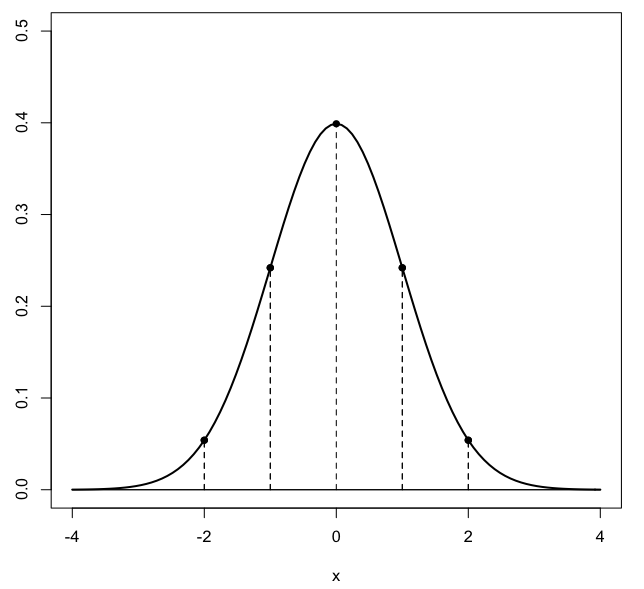
\includegraphics [scale=0.4] {gauss3.png} \end{center}
% \begin{bmatrix} a  &  b \\ c  &  d \end{bmatrix}
% \bigg |_

\begin{document}
\maketitle
\large
%\noindent
\begin{center} 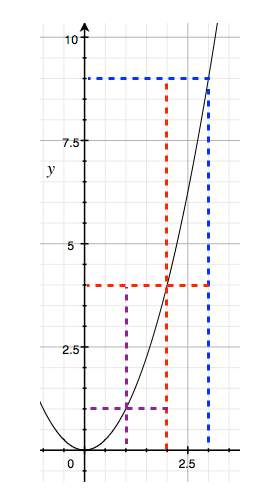
\includegraphics [scale=0.6] {area_x^2.png} \end{center}
The area under the curve is given by 
\[ \int_0^a x^2 dx = \frac{1}{3}x^3 \]
For $x=1,2,3,4 \cdots$, the values are $ \frac{1}{3}, \frac{8}{3},  \frac{27}{3},  \frac{64}{3} \cdots$.  I was curious about the pattern for areas above and below the curve, bounded by the rectangle drawn around $x,x^2$ for $x=n, x'=n+1$.

\noindent
Between $0$ and $1$, we have $\frac{1}{3}$ below and $\frac{2}{3}$ above.

\noindent
Between $1$ and $2$, we have $\frac{8}{3}-\frac{1}{3}-\frac{3}{3}=\frac{4}{3}$ below and $\frac{9}{3}-\frac{4}{3}=\frac{5}{3}$ above.

\noindent
Between $2$ and $3$, we have $\frac{27}{3}-\frac{8}{3}-\frac{12}{3}=\frac{7}{3}$ below and $\frac{15}{3}-\frac{7}{3}=\frac{8}{3}$ above.

\noindent
Between $3$ and $4$, we have $\frac{64}{3}-\frac{27}{3}-\frac{27}{3}=\frac{10}{3}$ below and $\frac{21}{3}-\frac{10}{3}=\frac{11}{3}$ above.


As $x$ grows larger, the areas above and below the line approach each other, always differing by $\frac{1}{3}$ and totalling $x^2-(x-1)^2 = 2x-1=(6x-3)/3$.



\end{document}  